\section{Introduction}
$K$-mer counting is a seemingly relatively straightforward process. Given a sequence $X = \{x_1,\dots,x_L\}$ of length $L$, for each position $i\in 1\leq i\leq \left(L-k+1\right)$ within the sequence, a sub-string is sliced from $[i,i+k)$. Where ``[" indicates inclusion, and ``)" indicates non-inclusive. A hash-map, or dictionary as known within Python, then saves the count for each $k$-mer as encountered in $X$. In many applications, the frequency of each $k$-mer would be calculated by dividing each $k$-mer count by the total number of $k$-mers, \emph{i.e.} $L-k+1$. 

SEEKR differs from this approach in that the algorithm adjusts from the non-uniformity of $k$-mers within our genome. Some $k$-mers are more, or less, frequent than others solely due to mononucleotide frequencies within the genome. Therefore, the enrichment for already common $k$-mers, or depletion of rare $k$-mers, are not informative unless it is known if they are significantly more enriched than background. To account for this, SEEKR calculates a $z$-score for each $k$-mer rather than a frequency.

The $z$-score is calculated by first calculating the $k$-mer frequencies within some reference set of sequences, \emph{e.g.} the transcriptome. From this reference set of $k$-mer frequencies, the mean frequency of each $k$-mer $\mu_j$ and the standard deviation of each $k$-mer $\sigma_j$ is calculated. 

For each $k$-mer frequency $j$ within a sequence $X$, $X_j$ has a $z$-score $X^*_j$: 

\begin{equation}
    X_j^* = \frac{X_j-\mu_j}{\sigma_j}
    \label{eq:zscore}
\end{equation}

We observed when studying the $k$-mer similarities between XIST and RSX that these $z$-scores were approximately log-normally distributed. For the analysis within that paper, we transformed $z$-scores as outlined in 2.X.X. However, we sought to perform a more rigorous analysis of different methodologies for adjusting $k$-mer counts. This chapter outlines the methods that we used and their results. 

\section{Results} 

\subsection{$k$-mer counts are log-normally distributed}

We observed that a primary challenge with estimating the correlation between highly repetitive regions of \emph{XIST} and other \emph{cis}-repressive lncRNAs was that the $k$-mer counts were heavily right-skewed. Pearson correlation is primarily intended to calculate the correlation between two normally distributed random variables. Spearman correlation can be used when this condition is not met, but a further observation we made was that the mode of the $k$-mer count distribution for any sequence or sub-sequence was 0, yielding artificially high correlations between any two given sequences. 

To correct for the right skewed distribution of $k$-mers across all sequences, we first confirmed that $k$-mer counts within lncRNAs are log-normally distributed (Figure \ref{fig:logdist}). The left panel of Figure \ref{fig:logdist} shows the marginal count distribution of $k$-counts summed over all possible $k$-mers, over all annotated human transcripts (Methods 4.x.x). We then log-transformed the data and observed an approximately normal distribution (Figure \ref{fig:logdist}), with the exception being the mode of the distribution was still a count of 0. This indicated that $k$-mer frequencies amongst all transcripts were log-normally distributed and that correcting for this in the SEEKR algorithm may yield better correlation estimates amongst transcripts. 
\begin{figure}[h!]
\centering
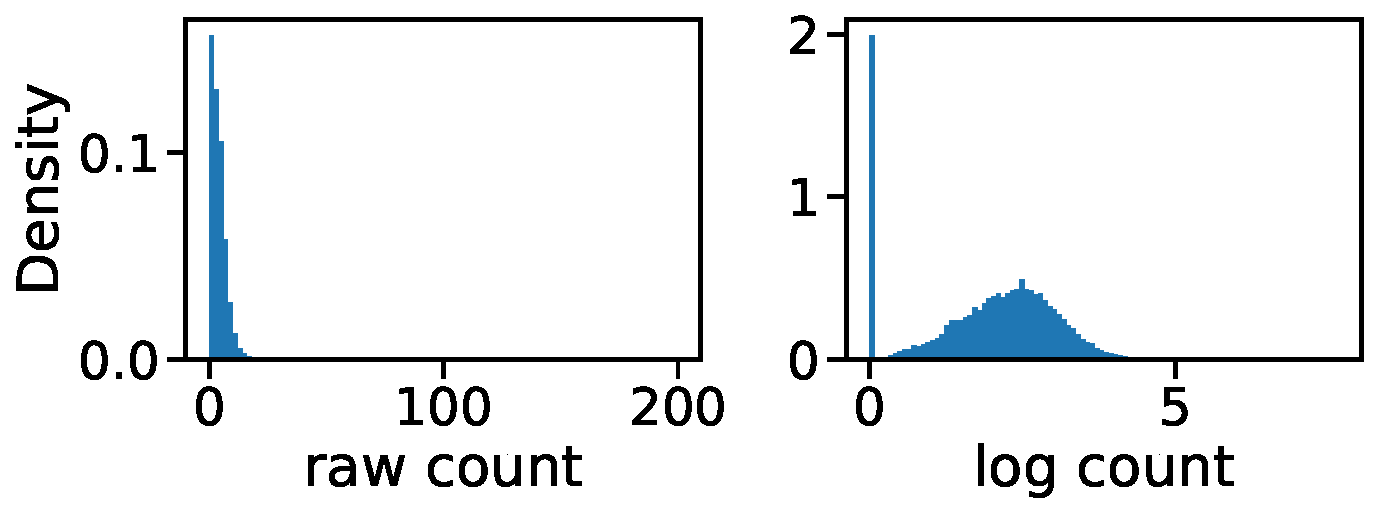
\includegraphics[width=\textwidth]{images/kmers_log_dist.pdf}
\caption{$k$-mer counts are log-normally distributed. A) The frequency of $k$-mer counts over all $k$-mers, over all annotated transcripts in the human genome. B) The distribution in (A), with log-transformed counts.}
\label{fig:logdist}
\end{figure}

\subsection{$k$-mer counting methodologies}

We then asked if we could devise a $k$-mer counting strategy that yielded more consistent estimates of correlations between two sequences, in a way that is sensible and mathematically tractable. The primary difficulty is the addition of a $z$-score calculation step within SEEKR, which transforms the data in a way that suppresses the influence of naturally frequent or depleted $k$-mers within a reference set, \emph{e.g.} the transcriptome. 

Within our \emph{Rsx} analysis in Chapter 2, we originally noticed that the $z$-scores themselves were log-normally distributed, and so we log-transformed the $z$-scores after shifting all values by equation \ref{eq:seekrrsx} (Sprague et al, 2019).

\begin{equation}
M_{ij}^* = \log_2{\left(M_{ij} + |\min{M}|+1\right)}
\label{eq:seekrrsx}
\end{equation}


Where $M$ is the SEEKR $z$-score matrix, $i$ is the row, $j$ is the column ($M_{ij}$ is then the coordinates of a single data point in $M$), and $\min{M}$ is the smallest value in the matrix $M$. This translation of the data allows for the calculation of the log. An issue with this methodology, however, is that there is no clear best choice of value to add to each data point in $M$, due to the log-transform. The goal, therefore, was to add the smallest possible value to each data-entry without destroying the linear relationship between row vectors. Each row within a SEEKR matrix represents the vector of $k$-mer frequencies within a single sequence, and the correlation step in SEEKR calculates the Pearson correlation between all pair-wise combinations of rows within $M$.

Below, we iterate through a series of algorithms for generating the final SEEKR matrix from which correlations will be calculated. 

\subsubsection{Method 1. Kirk et al. 2018}

The first method we outline is the original algorithm published in \emph{Kirk et al.}. Here, we first count the occurrence of each $k$-mer in a sequence. This count is then normalized to a per-kB count by dividing each $k$-mer count by the length of the sequence and multiplying by 1000. This process is then repeated for a reference set of sequences, \emph{e.g.} the transcriptome, and the mean frequency and standard deviation for each $k$-mer over the reference set are calculated. From there, each frequency count in the SEEKR frequency matrix is transformed using Equation \ref{eq:zscore}. 

\begin{table}[h]
\begin{center}
\begin{tabular}{llllll}
&MXA & MXB                   & MXC                  & HXD                   & MXE                                         \\
KR1 & -0.048 & 0.266   & 0.001 & 0.146    & -0.117 \\
KR2 & 0.085   & -0.089  & -0.111  & -0.024 & 0.147  \\
KR3 & -0.041 & -0.119   & -0.009 & -0.021 & 0.267   \\
KR4 & 0.180   & -0.114 & -0.081  & 0.087   & 0.294 
\end{tabular}
\caption{SEEKR Pearson correlations between the tandem repeats of \emph{Xist} and \emph{Rsx}. Correlations were calculated as in \emph{Kirk et al.}, 2018.}
\label{tbl:kmers1}

\end{center}
\end{table}

From here, the pair-wise correlations of each sequence's $k$-mer profile, \emph{i.e.} the row vector of $k$-mer $z$-scores, are calculated. For each of the methods outlined in this chapter, we compare the tandem repeats of \emph{XIST} against the tandem repeats of \emph{Rsx} as in \emph{Sprague et al.}. The correlations for this algorithm are shown in Table \ref{tbl:kmers1}.

\subsubsection{Method 2. Sprague et al. 2019}

\begin{table}[h]
\begin{center}
\begin{tabular}{llllll}
&MXA & MBX                  & MXC                  & HXD                  & MXE                                        \\
KR1 & -0.021 & 0.325   & 0.038 & 0.193   & -0.163 \\
KR2 & 0.084  & -0.122  & -0.122 & -0.013 & 0.145  \\
KR3 & -0.077   & -0.093 & 0.014 & -0.023 & 0.249   \\
KR4 & 0.210   & -0.114 & -0.068 & 0.112   & 0.398
\end{tabular}
\caption{SEEKR Pearson correlations between the tandem repeats of \emph{Xist} and \emph{Rsx}. Correlations were calculated as in \emph{Sprague et al.}, 2019.}
\label{tbl:kmers2}

\end{center}
\end{table}

The second method outlined is the algorithm published in \emph{Sprague et al.}. The $k$-mers are counted exactly as in \emph{Kirk et al.}, however we additionally calculated the $log_2$ of the $z$-scores using Equation \ref{eq:seekrrsx}. Tandem repeat comparisons that were highly correlated as in Method 1 saw large increases in correlation using this method, whereas uncorrelated regions saw little change (Table \ref{tbl:kmers2}). 




\subsubsection{Method 3. Row-wise addition to z-scores}

A concern when translating data, as in Equation \ref{eq:seekrrsx}, is the unequal effect it has when calculating the log of the data. Typically, Pearson correlation is translation invariant, \emph{i.e.} the addition of any constant to all elements of a vector does not affect its correlation with another vector. This is because the calculation of the Peasron correlation involves 0-mean centering each vector, which negates the addition or multiplication of any constant. Another intuition is that moving a scatter plot around on a graph changes the location of the data points, but it doesn't change the relative relationship between data points (slope of best fit). 

\begin{table}[ht]
\begin{center}
\begin{tabular}{llllll}
&MXA & MXB                   & MXC                  & HXD                  & MXE                                  \\
KR1 & -0.017 & 0.327   & 0.042  & 0.197    & -0.163 \\
KR2 & 0.088   & -0.124 & -0.120 & -0.009 & 0.147 \\
KR3 & -0.079  & -0.090 & 0.016 & -0.022 & 0.246 \\
KR4 & 0.214    & -0.110 & -0.066  & 0.115   & 0.404
\end{tabular}
\caption{SEEKR Pearson correlations between the tandem repeats of \emph{Xist} and \emph{Rsx}. Correlations were calculated as in \emph{Sprague et al.}, 2018., except that instead of the minimum of the $z$-score matrix being added, the minimum of each row was added to all values within the row.}
\label{tbl:kmers3}
\end{center}
\end{table}

However, the inclusion of a log-transformation step alters the linear relationship of the data depending on how far the data is from 0. Therefore, it is ideal to add the smallest possible constant to each entry in the matrix. \emph{Sprague et al.} added the minimum of the entire matrix to each $z$-score, however adding the minimum of each row to all values within that row allows for the addition of the smallest possible value such that the log can be taken, without altering the relationship between the $k$-mer counts within a given sequence. The results were similar to those in Method 2, except with further increases in correlation between high correlated domains such as KR4-MXE and KR1-MXB (Table \ref{tbl:kmers3}). 


\subsubsection{Method 4: Column-wise addition to z-scores}

To illustrate the point that the value added to the SEEKR matrix must be constant within a row, here we repeat what was done in Method 3, but instead of adding the minimum of each row to all values within that row, we take the minimum of each column and add that value to each element within the column.

\begin{table}[ht]
\begin{center}
\begin{tabular}{llllll}
&MXA & MXB                  & MXC                   & HXD                 & MXE                                      \\
KR1 & -0.048 & 0.348    & 0.093 & 0.284  & -0.098 \\
KR2 & 0.057  & -0.046 & 0.034 & 0.201 & 0.261  \\
KR3 & -0.061 & -0.015 & 0.144 & 0.173 & 0.347  \\
KR4 & 0.147   & -0.094  & 0.044 & 0.241 & 0.451 
\end{tabular}
\caption{SEEKR Pearson correlations between the tandem repeats of \emph{Xist} and \emph{Rsx}. Correlations were calculated as in \emph{Sprague et al.}, 2018., except that instead of the minimum of the $z$-score matrix being added, the minimum of each column was added to all values within the column.}
\label{tbl:kmers4}
\end{center}
\end{table}
As an example, consider the hypothetical SEEKR $z$-score matrix in Table \ref{tbl:ex1}. After applying the transformation described in this section, all values are greater than 0 which allows for the log-transform of the data (Table \ref{tbl:ex2}. However, the $k$-mer frequencies within each sequence have become jumbled. Consider the relationship between A and T in seq1. Prior to the transformation, T was clearly depleted relative to A in seq1, with $z$-scores of -2 and 0 respectively. 
\begin{table}[h!]
\begin{center}
\begin{tabular}{lllll}
&A & T                   & C                  & G                                                    \\
seq1 & 0 & -2   & 5  & -3 \\
seq2 & 0   & 1 & 3 & -2 
\end{tabular}
\caption{A hypothetical SEEK $z$-score matrix.}
\label{tbl:ex1}
\end{center}
\end{table}
After the transformation, the SEEKR matrix is now indicating that A and T are equally frequent in seq1. Likewise, G was depleted relative to A in both seq1 and seq2, but after the operation is now enriched relative to A.  This operation therefore does not make sense, as we are only trying to move the data to be positive, such that we can calculate the log. While the correlations look promising in Table \ref{tbl:kmers4}, the scatter plots of the $k$-mer counts show that  significant aberration has been introduced to the data relative to Methods 1,2 and 3 (Figure \ref{fig:2plots}). 


\begin{table}[h!]
\begin{center}
\begin{tabular}{lllll}
&A & T                   & C                  & G                                                    \\
seq1 & 1 & 1   & 7  & 1 \\
seq2 & 1   & 4 & 5 & 2  
\end{tabular}
\caption{The same matrix as in Table \ref{tbl:ex1} but transformed by adding the minimum of each column to all values within that column, then adding 1 such that all values are greater than 0.}
\label{tbl:ex2}
\end{center}
\end{table}

\begin{figure}[h]
\centering
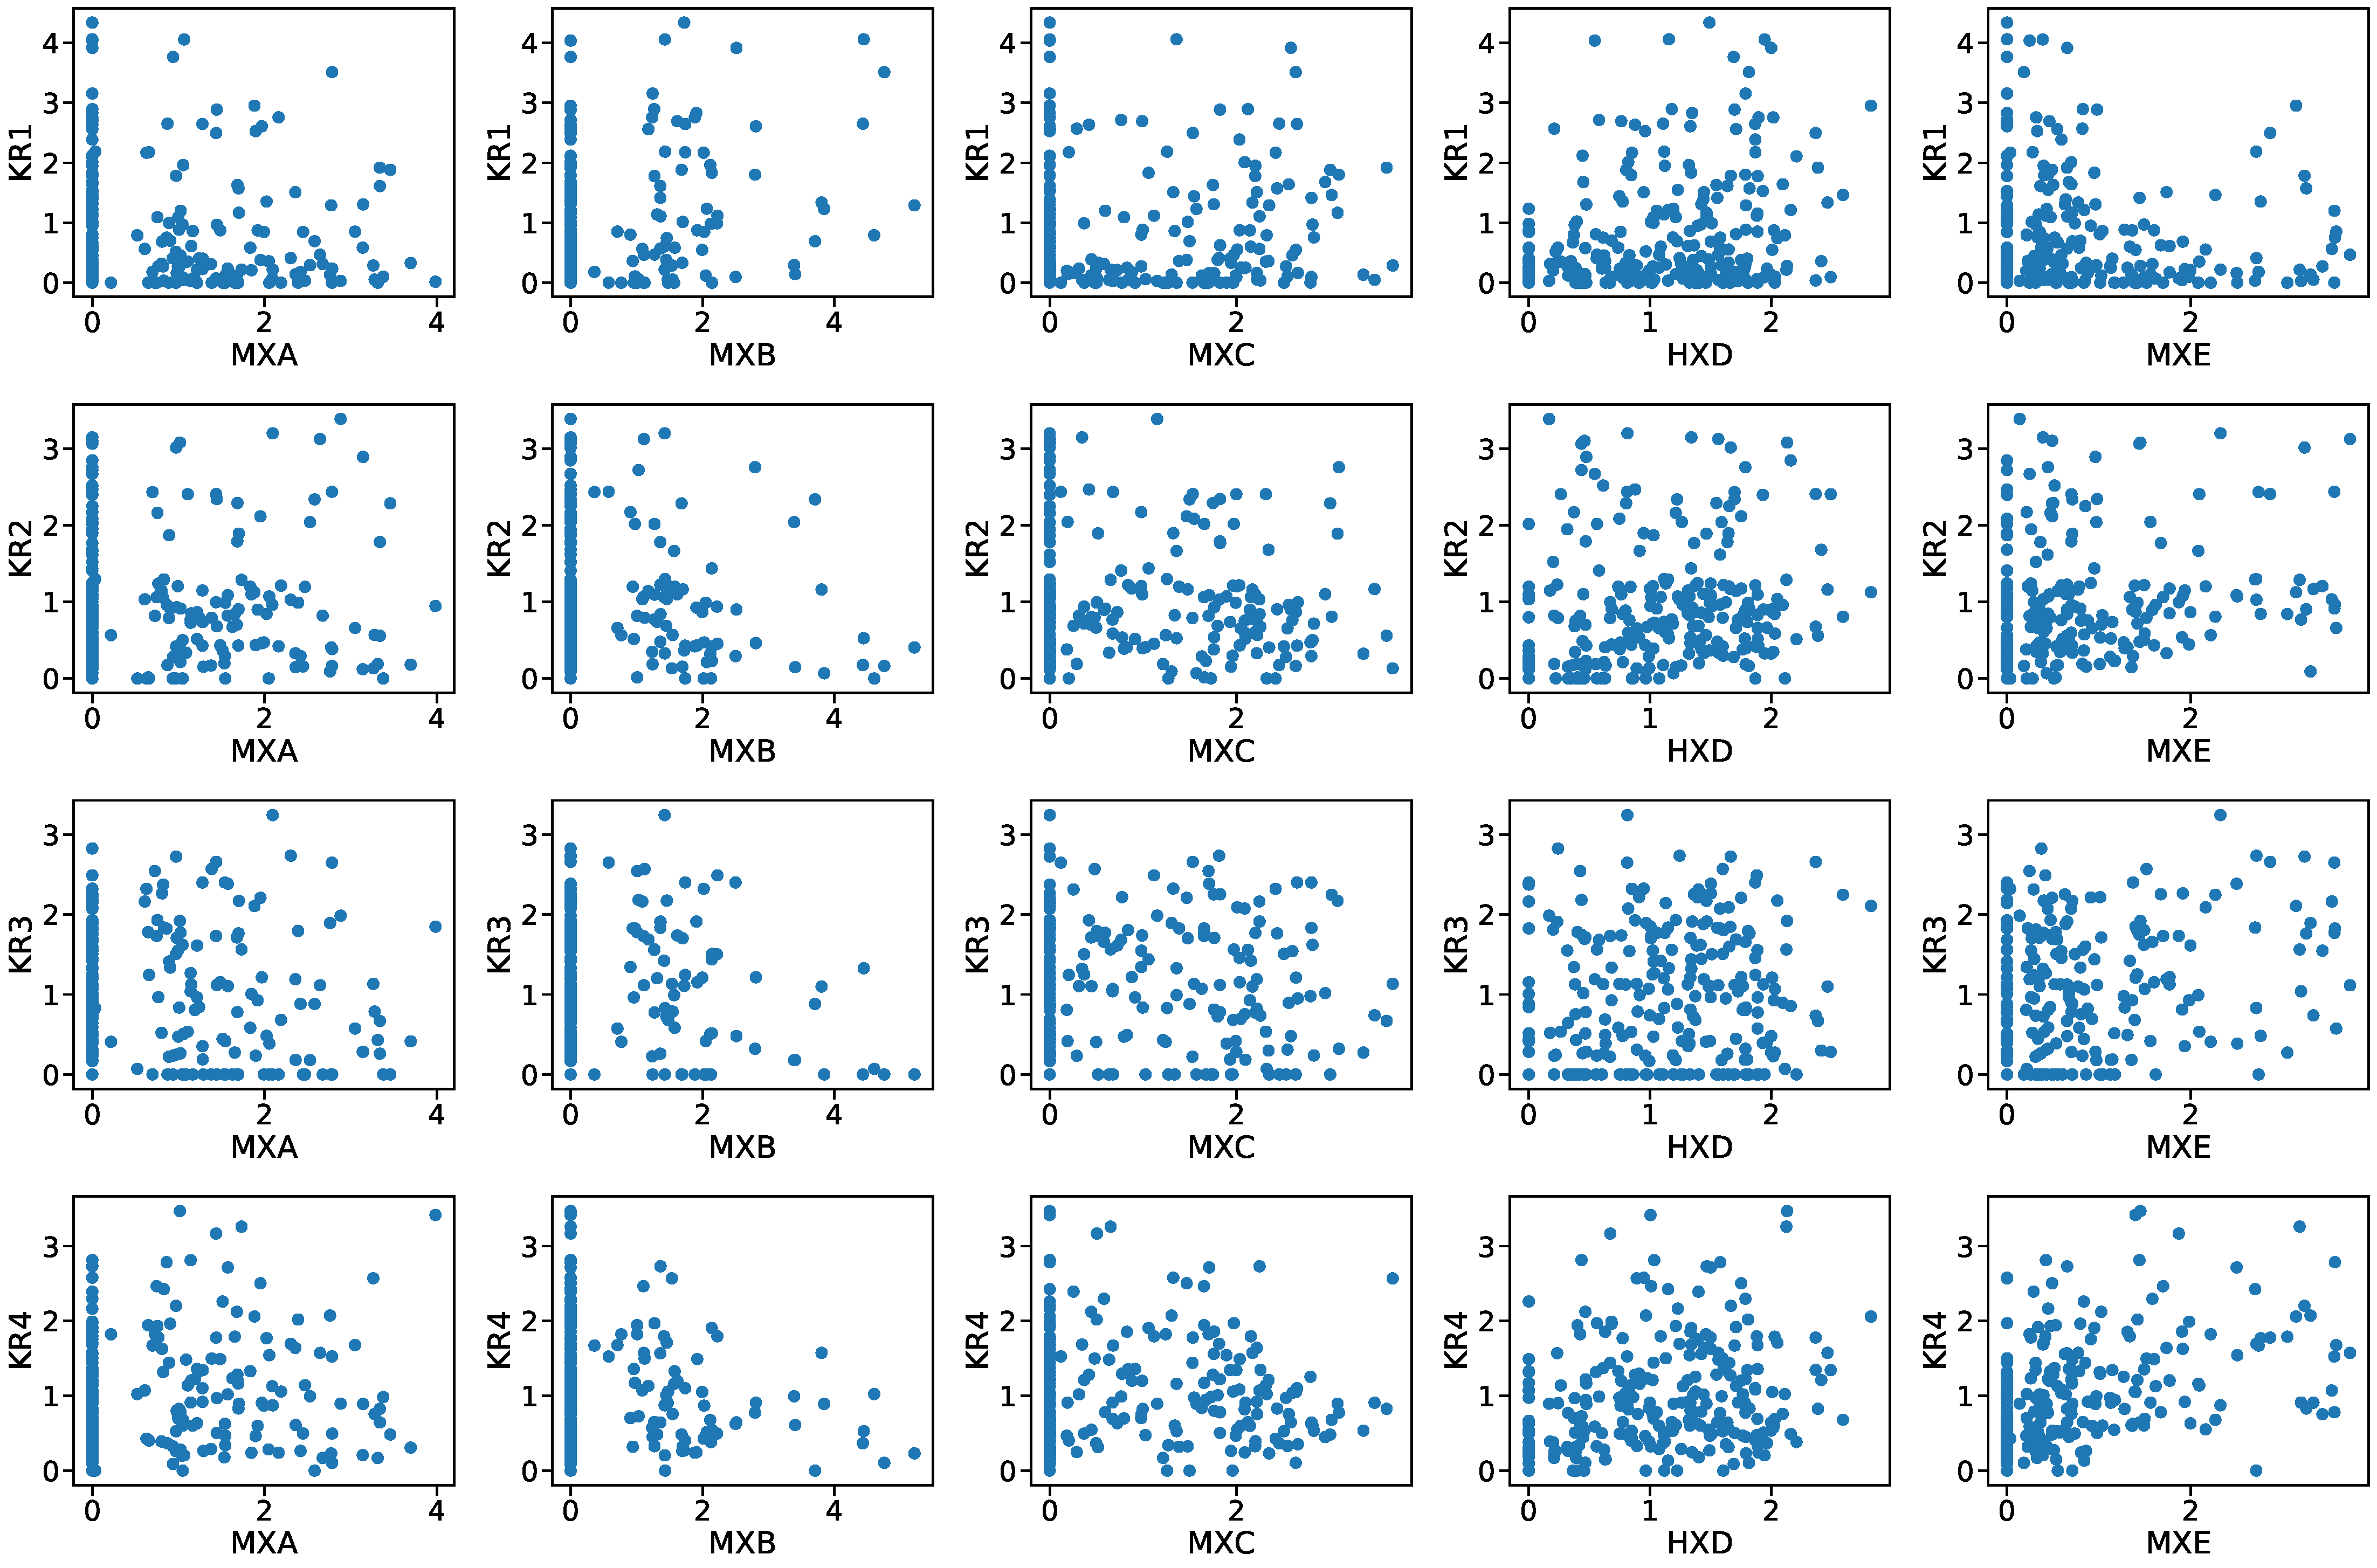
\includegraphics[width=\textwidth]{images/2_figs.pdf}
\caption{Scatter plots of SEEKR $z$-scores for all pair-wise comparisons between MXA,MXB,HXD,MXE and KR1,KR2,KR3, and KR4 using Method 4. Each dot represents a $k$-mer $z$-score for both transcripts being compared (x,y axis).}
\label{fig:2plots}
\end{figure}

\subsubsection{Method 5: Pseudo-count to raw counts}

A more natural transformation of the data is to take the logarithm of the raw count data, which is guaranteed to be $\geq 0$. A potential downside with this approach is that adding 1 to raw counts has a differential effect on sequences of different lengths, \emph{i.e.} adding +1 to the count of all $k$-mers in a sequence that is 200bp long has a larger effect on the frequencies than a 10,000bp sequence. Therefore, we tried two different approaches. In Method 5, we added +1 to the raw counts of the data, length normalized the counts, and then took the log-transform, followed by $z$-score calculation as in \emph{Kirk et al.} (Table \ref{tbl:kmers5}).

\begin{table}[ht]
\begin{center}
\begin{tabular}{llllll}
&MXA & MXB                  & MXC                  & HXD                  & MXE                                         \\
KR1 & -0.068 & 0.232    & 0.024  & 0.181   & -0.179 \\
KR2 & -0.074 & -0.295 & -0.087 & 0.071  & 0.126  \\
KR3 & -0.170 & -0.170 & 0.063   & 0.001 & 0.205  \\
KR4 & 0.119  & -0.175  & -0.014 & 0.148   & 0.387
\end{tabular}
\caption{SEEKR Pearson correlations between the tandem repeats of \emph{Xist} and \emph{Rsx}. Correlations were calculated adding a pseudo-count to the raw count data (Method 5).}
\label{tbl:kmers5}
\end{center}
\end{table}

\subsubsection{Method 6: Length normalized pseudo-count}
The second method was to add 1 after length normalizing the $k$-mer counts per kB, effectively making the pseudo-count equivalent between transcripts of different lengths, and then going through SEEKR as before. The results are shown in Table \ref{tbl:kmers6}. This latter method of adding a pseudo-count posterior to length normalization is the method we chose to continue using with SEEKR going forward, as the mathematics are straigt forward and are best suited to the data at hand, as well as yielding strong results between regions known to share similar function and $k$-mer frequencies (Figure \ref{fig:9plots}). 

\begin{table}[ht]
\begin{center}
\begin{tabular}{llllll}
&MXA & MXB                   & MXC                  & HXD                  & MXE                                        \\
KR1 & -0.013 & 0.335  & 0.059  & 0.200  & -0.163 \\
KR2 & 0.039   & -0.152 & -0.080  & -0.007 & 0.135  \\
KR3 & -0.102   & -0.067 & 0.076  & -0.025 & 0.220   \\
KR4 & 0.249   & -0.078 & 0.015 & 0.150  & 0.431 
\end{tabular}
\caption{SEEKR Pearson correlations between the tandem repeats of \emph{Xist} and \emph{Rsx}. Correlations were calculated using a length normalized pseudo-count (Method 6).}
\label{tbl:kmers6}
\end{center}
\end{table}

\begin{figure}[h]
\centering
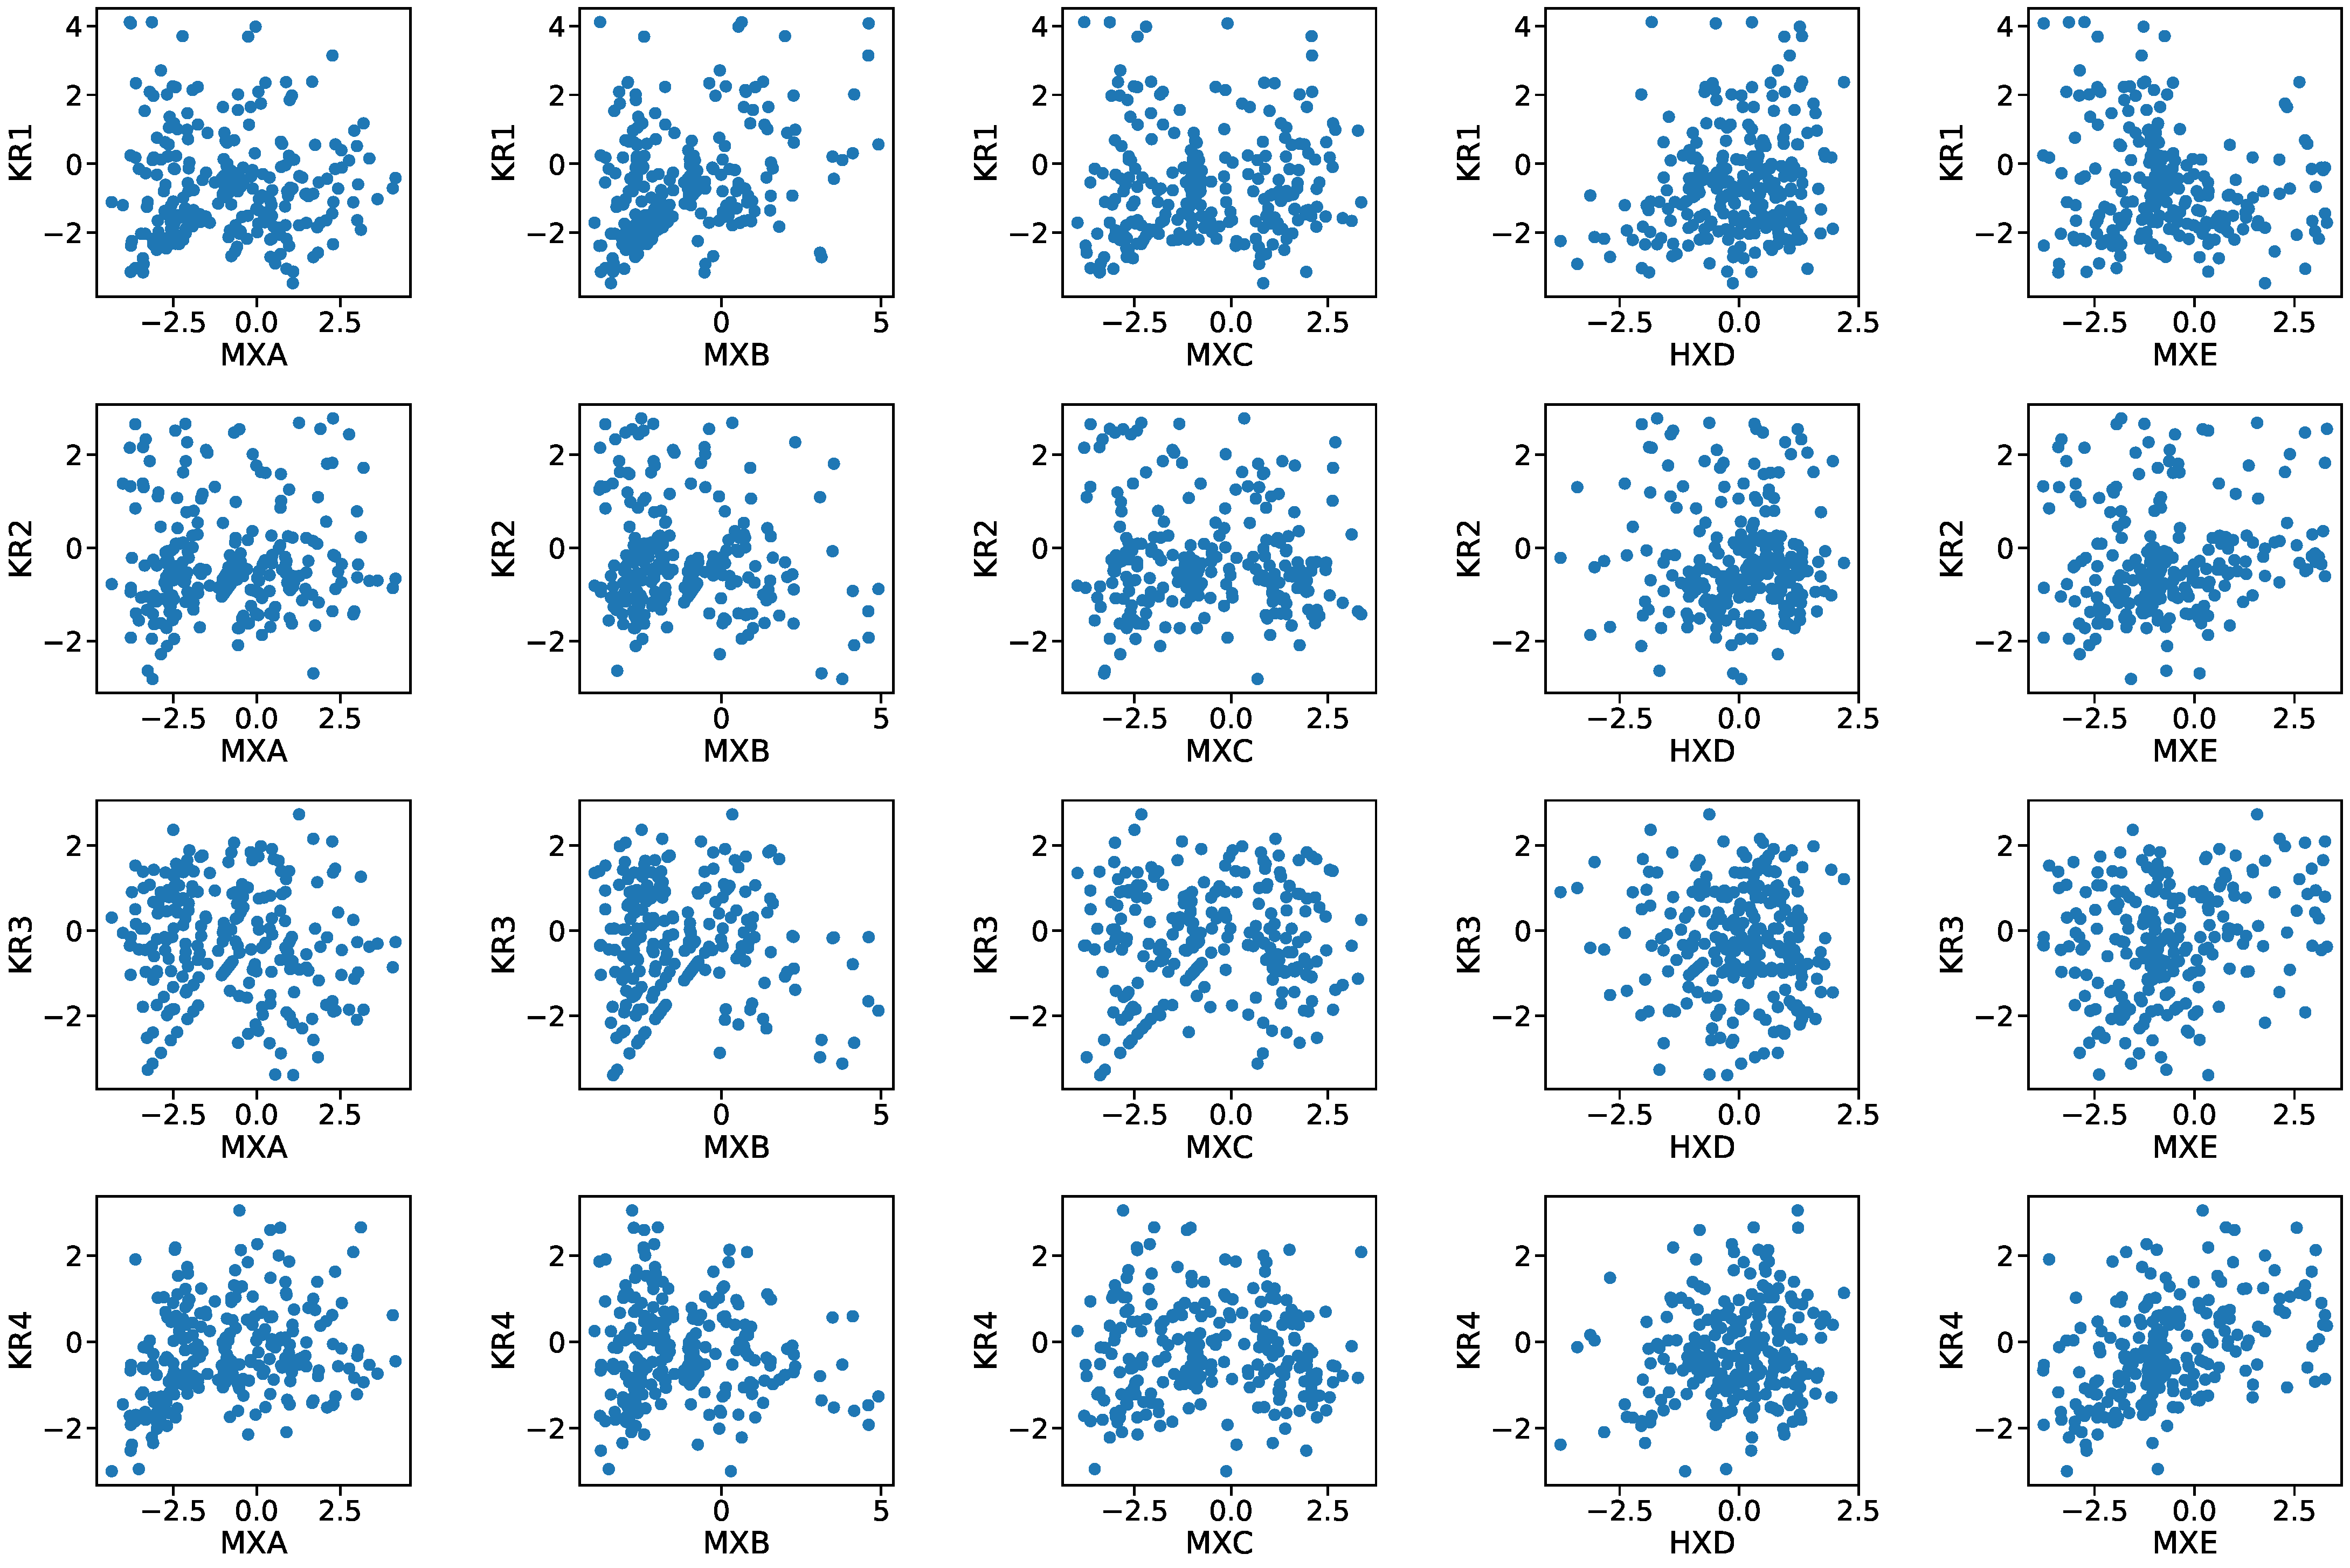
\includegraphics[width=\textwidth]{images/9_figs.pdf}
\caption{Scatter plots of SEEKR $z$-scores for all pair-wise comparisons between MXA,MXB,HXD,MXE and KR1,KR2,KR3, and KR4 using Method 6. Each dot represents a $k$-mer $z$-score for both transcripts being compared (x,y axis).}
\label{fig:9plots}
\end{figure}

\clearpage

\section{Methods}

\subsection{$k$-mer count distributions}

For a given sequence, \emph{e.g.}``seq1", we counted how many times we observed each $k$-mer. This yields a vector representing $\{c_{AAA},c_{AAT},\dots\,c_{GGG}\}$, where $c_{kmer}$ is the number of observed counts for that $k$-mer. We then calculated the frequency distribution of counts in a sequence, over all $k$-mers. \emph{E.g.}, if the $k$-mers AAA and GGG had counts $c_{AAA} = 5$ and $c_{GGG} = 5$, and no other $k$-mers had a count of 5 in ``seq1", then we would record a frequency of 2 for the number of times we observed a count of 5 in ``seq1". These observed frequencies were calculated for each transcript and then summed, \emph{e.g.} if we observed a count of 5 twice in ``seq1" and 10 times in ``seq2", then the marginal frequency of a count of 5 over those two sequences is 15.

$$
P(\texttt{frequency}) = \sum_{\texttt{k-mers}}{\sum_{\texttt{sequences}}{P(\texttt{frequency,sequences,k-mers)}}}
$$

\subsection{SEEKR Data Sources}
For each of the analyses above, we used the following transcript annotations. For \emph{XIST}, we used Mouse A-repeat (MXA), mouse B-repeat (MXB), human D-repeat (HXD), and mouse E-repeat (MXE) as annotated in \cite{Brockdorff10TheNucleus.}. For the \emph{Rsx} repeats, we used the koala \emph{Rsx} 1,2,3, and 4 repeats as defined in \cite{Sprague2019NonlinearDomains}. For the reference set of sequences within SEEKR, used the GENCODE (M14) annotated set of spliced lncRNA transcripts in the mouse transcriptome. 


\begin{singlespace}
\printbibliography
\end{singlespace}